\begin{figure*}[h]
    \centering
    \subfloat[Quenched (AR).]{%
        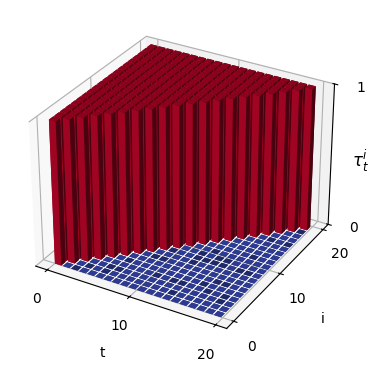
\includegraphics[width=0.23\textwidth]{figs/Qwench.png}%
        \label{figure:tau:quenched}
    }
    \hfill
    \subfloat[Flat annealing.]{%
        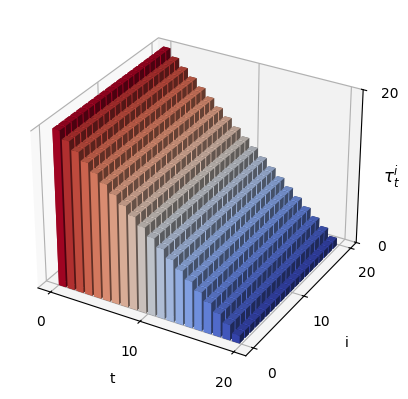
\includegraphics[width=0.23\textwidth]{figs/Flat.png}%
        \label{figure:tau:flat}
    }
    \hfill
    \subfloat[Block annealing.]{%
        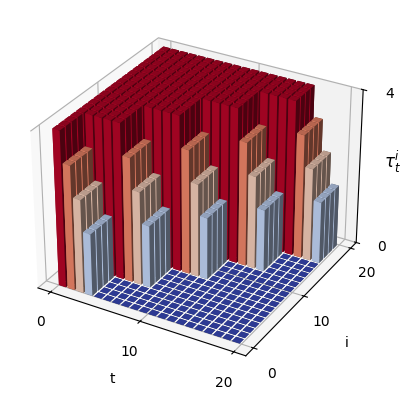
\includegraphics[width=0.23\textwidth]{figs/Block.png}%
        \label{figure:tau:block}
    }
    \hfill
    \subfloat[Slide annealing.]{%
        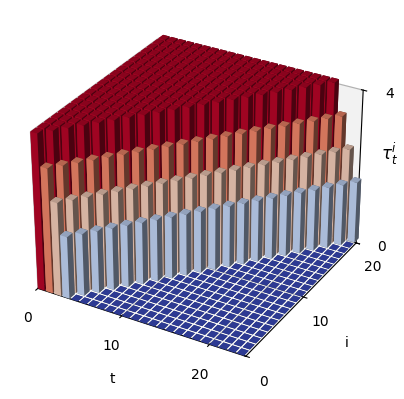
\includegraphics[width=0.23\textwidth]{figs/Slide.png}%
        \label{figure:tau:slide}
    }
    %
    \caption[shorttitle]{%
        Fathi et al.~\cite{fathi_unifying_2025} introduce $\boldsymbol{\tau}$-\emph{hyperschedules}, subjecting different token positions $i$ to different noise levels (red: high; blue: low) at different generation step $t$. 
        (a) Standard AR models (e.g., GPT) determine tokens one by one, ``quenching'' each of them to full determination in a single step, and can be seen as an extreme case of a diffusion model. 
        (b) Standard diffusion models (e.g., SEDD) gradually anneal all tokens independently of position. 
        (c) Block-wise annealing for blocks of width $\omega=4$. 
        (d) Sliding window annealing (``smoothed'' AR) with window width $\omega=4$. These last two combine properties of both AR and diffusion.%
    }
    \label{fig:four_subfigs}
\end{figure*}

We organize diffusion language models (DLLMs) along four orthogonal axes: \emph{Markovity}, \emph{Guidance}, \emph{Annealing Method}, and \emph{Time Conditioning}.  The following explains the foundational works that defined each criterion.

\subsection{Markovian vs.~Non-Markovian Sampling}
The distinction between Markovian and non-Markovian diffusion processes in generative modeling goes back to the original DDPM framework. The work formulates a \textbf{Markovian} forward and reverse noising chain \cite{sohl-dickstein_deep_2015}. The seminal work on \textbf{non-Markovian} diffusion processes was introduced in the Denoising Diffusion Implicit Models (DDIM) paper. The authors generalized the DDPM’s Markov chain to a broader family of trajectories that retain the same training objective but allow deterministic or accelerated sampling \cite{song_denoising_2020}.

\subsection{Classifier-Based vs.~Classifier-Free Guidance}
\textbf{Classifier-based guidance}—reweighting diffusion samples with an external classifier’s gradients—was popularized in “Improved Denoising Diffusion Probabilistic Models,” showing how to trade off sample diversity and fidelity via classifier gradients during sampling \cite{nichol_improved_2021}.  Shortly thereafter, \textbf{classifier-free guidance} was proposed by Ho and Salimans, eliminating the need for a separate classifier by jointly training conditional and unconditional diffusion models and interpolating between their score estimates \cite{ho_classifier-free_2022}.


\subsection{Annealing Method (Noise Scheduling)}
The need to choose a noise schedule for the forward diffusion process was first formalized in the original DDPM paper, which proposed a fixed variance schedule $\{\beta_t\}$ and showed how it affects both likelihood and sample quality \cite{ho_denoising_2020}. Subsequent work (“Improved DDPM”) explored alternative schedules (e.g.\ cosine) and adaptive variance learning for faster convergence and fewer sampling steps \cite{nichol_improved_2021}.

\subsection{Time Conditioning vs.~Time-Agnostic Kernels}
In standard DDPMs, the denoiser is conditioned on an explicit \textbf{timestep embedding}, a mechanism first described in the DDPM framework to inform the network of the current noise level \cite{ho_denoising_2020}.  In contrast, the concept of \textbf{time-agnostic} diffusion—where transitions do not depend on an explicit $t$ embedding—has been introduced in the discrete “absorbing” diffusion models, notably in Hoogeboom \emph{et al.}’s D3PM work, which defines absorbing‐state kernels without explicit timestep conditioning \cite{hoogeboom_structured_2021}.

